\documentclass[11pt,letterpaper,twocolumn]{article}

\usepackage[utf8]{inputenc}
\usepackage[spanish]{babel}
\usepackage{float}
\usepackage[table]{xcolor}
\usepackage{mwe}
\usepackage{charter}
\usepackage{afterpage}
\usepackage{amsmath}
\usepackage{appendix}
\usepackage[hidelinks]{hyperref}
\usepackage{ragged2e}
\usepackage{array}
\usepackage{etoolbox}
\usepackage{fancyhdr}
\usepackage{booktabs}
\usepackage{arydshln}
\usepackage[justification=justified,singlelinecheck=false,labelfont=bf,format=plain]{caption}
\usepackage[justification=justified,singlelinecheck=false,labelfont=bf,format=plain]{subcaption}
\usepackage{enumitem}
\usepackage[bottom=2.5cm,top=2.0cm,left=2.0cm,right=2.0cm]{geometry}
\usepackage{graphicx}
\usepackage{indentfirst}
\usepackage{mathtools}
\usepackage{multirow}
\usepackage{pdfpages}

\usepackage{subfiles}
\usepackage[compact]{titlesec}
\usepackage{blindtext}
\usepackage{stfloats}
\usepackage{lipsum} 


\renewcommand{\familydefault}{\rmdefault}

\newcommand\blankpage{
    \null
    \thispagestyle{empty}
    \addtocounter{page}{0}
    \newpage}

\newcolumntype{L}[1]{>{\raggedright\let\newline\\arraybackslash\hspace{0pt}}m{#1}}
\newcolumntype{C}[1]{>{\centering\let\newline\\arraybackslash\hspace{0pt}}m{#1}}
\newcolumntype{R}[1]{>{\raggedleft\let\newline\\arraybackslash\hspace{0pt}}m{#1}}

    \setlist[itemize,1]{label=$\bullet$}
    \setlist[itemize,2]{label=$\circ$}
    \setlist[itemize,3]{label=$-$}
    \setlist{nosep}

\setlength{\columnsep}{20pt}

\titlelabel{\thetitle.\quad}

\pagestyle{fancy}
\fancyhf{}
      
\fancyfoot{}
\fancyfoot[C]{\thepage} % page
\renewcommand{\headrulewidth}{0mm} % headrule width
\renewcommand{\footrulewidth}{0mm} % footrule width

\makeatletter
\patchcmd{\headrule}{\hrule}{\color{black}\hrule}{}{} % headrule
\patchcmd{\footrule}{\hrule}{\color{black}\hrule}{}{} % footrule
\makeatother

\definecolor{blueM}{cmyk}{1.0,0.49,0.0,0.47}

%%%%%%%%%%%%%%%%%%%%%%%%%%%%%%%%%%%%%%%%%%%%%%%%%%%%%%%%%%%%%%%%%%%%%%%%%%%%%%%%%%%%%%%%%%%%%%%%%%%%%%%%%%%%%%%%%%%%%%%%%%%%%%%%%%%%%%%%%%%%%%%%%%%%%%%%%%%%%%%%%%%%%%%%%%%%%%%%%%%%%%%%%%%%%%%%%%%%%%%%%%%%%%
%%%%%%%%%%%%%%%%%%%%%%%%%%%%%%%%%%%%%%%%%%%%%%%%%%%%%%%%%%%%%%%%%%%%%%%%%%%%%%%%%%%%%%%%%%%%%%%%%%%%%%%
%%%%%%%%%%%%%%%%%%%%%%%%%%%%%%%%%%%%%%%%%%%%%%%%%%%%%%%%%%%%%%%%%%%%%%%%%%%%%%%%%%%%%%%%%%%%%%%%%
             %elija el que corresponda ejemplo :  Modular : I
%%%%%%%%%%%%%%%%%%%%%%%%%%%%%%%%%%%%%%%%%%%%%%%%%%%%%%%%%%%%%%%%%%%%%%%%%%%%%%%%%%%%%%%%%%%%%%%%%
\begin{document}
\twocolumn[\begin{@twocolumnfalse}


\begin{center}
	
\begin{minipage}{0.75\textwidth}
\vspace{5mm}
\centering{
	\hspace{2.4cm}	
\includegraphics[scale=0.1]{img/logo.png} \newline
\Large{\textbf{Práctica 3. Interferómetros de Michelson y Fabry-Perot}} %
    \vspace{3mm}
    \\
    \large{Alberca Berbel, Fernando \\ Gómez Gómez, José Luis \\ Martín Romero, Álvaro} % Si solo hay un autor borrar el apartado sin borrar el ultimo }
    \vspace{2mm}
    
    \large{Profesor encargado: Prof. Jorge Hidalgo Aguilera} \newline
    %Si solo hay un asesor borrar el 1'' y el apartado de Asesor 2
     \textit{Departamento de Física, Laboratorio de Óptica, Universidad de Córdoba\newline }
    \vspace{1mm} 
    
    \today % FECHA
}
\end{minipage}

\end{center}
\small

\vspace{11pt}

\end{@twocolumnfalse}]
%%%%%%%%%%%%%%%%%%%%%%%%%%%%%%%%%%%%%%%%%%%%%%%%%%%%%%%%%%%%

\section{Introducción}%
En esta práctica se estudia el fenómeno de interferencias que se produce en los interferómetros de Michelson y Fabry-Perot. El patrón de ondas producido por ambos interferómetros son unas coronas circulares difusas concéntricas iluminadas para las interferencias constructivas y oscuras para las interferencias destructivas. \\
\\
Al modificar la posición de uno de los espejos de los interferómetros, se modifica un camino óptico uno de los rayos desdoblados, esto permite calcular la longitud de onda de la fuente emisora. \\
\\
También se puede modificar el camino óptico cambiando la densidad del medio por donde pasa uno de los haces. De esta forma se puede deducir la dependencia del índice de refracción del aire con la presión.
\vfill\hfill 
\begin{figure}[H]
    \centering
    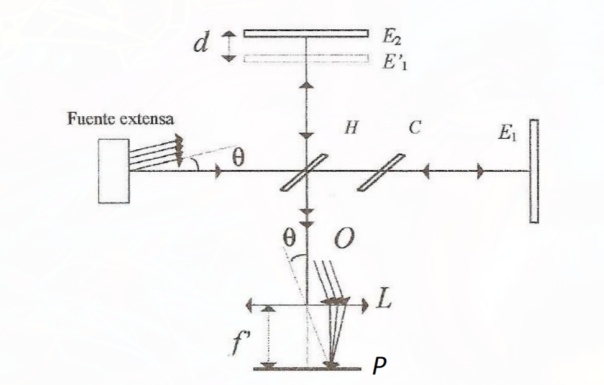
\includegraphics[width=0.6\textwidth]{img/int1.png}
    \caption{Esquema del interferómetro de Michelson}
    \label{fig:img-int1-png}
\end{figure}
\begin{figure}[H]
    \centering
    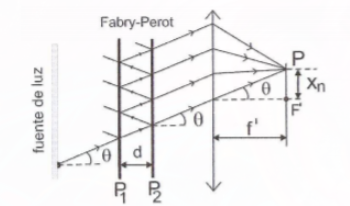
\includegraphics[width=0.5\textwidth]{img/int2.png}
    \caption{Esquema del funcionamiento del interferómetro de Fabry-Perot}
    \label{fig:img-int2-png}
\end{figure}
\section{Análisis de variables}%
\begin{figure}[H]
    \centering
    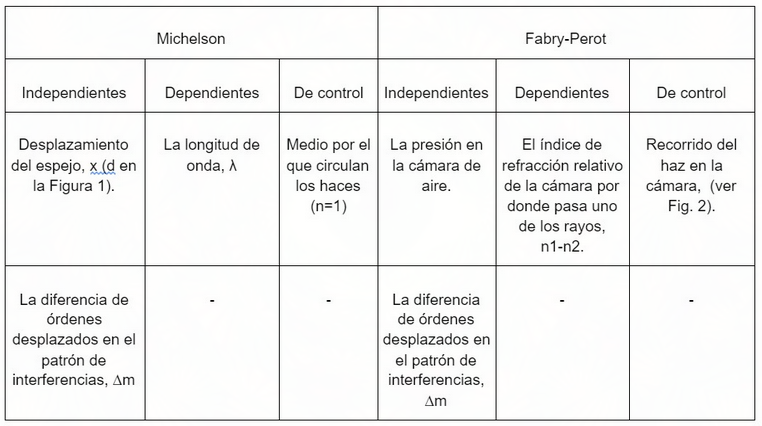
\includegraphics[width=0.5\textwidth]{img/variables.png}
    \label{fig:img-variables-png}
\end{figure}
\subsection{Relaciones entre variables}
\begin{figure}[H]
    \centering
    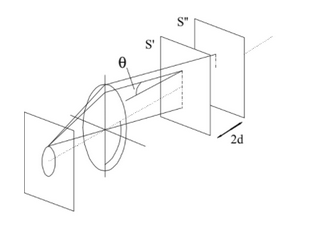
\includegraphics[width=0.4\textwidth]{img/relvar.png}
    \caption{Detalle del patrón resultado}
    \label{fig:i}
\end{figure}
    Desde la pantalla en el final del recorrido, P (fig. 1), todo se observa como si la luz proviniese de dos fuentes, en S' y S'', imágenes de la fuente S en los espejos E1 y E2, respectivamente. Por la configuración del sistema óptico, tendremos un máximo en la interferencia cuando:
    \begin{equation}
        2nd\cos\theta=m\lambda
    \end{equation}
Con $m=0,1,2\ldots$ \\
\\
Para el máximo central, $\cos \theta =1$. Si el $ E_2$ recorre una distancia $x$, el nuevo orden del máximo central tiene que cumpli:
\begin{equation}
    2x=\Delta m \lambda 
\end{equation}
\subsection{Medida del índice de refracción}
Para bajas presiones, el índice de refracción del aire depende linealmente de la presión P, de modo que vale 1 para presión nula (vacío). Por tanto, podemos expresar el índice de refracción del aire como: 
\begin{equation}
    n=mP+1  
\end{equation}
Siendo $d$ la distancia que recorre el haz en la cámara, se cumple que el número de longitudes de onda que caben en la cámara es $\frac{d}{\lambda}$. La diferencia de camino óptico al variar la presión al recorrer la cámara dos veces viene dado por la expresión:
\begin{equation}
    D=\frac{2d}{\lambda_2}-\frac{2d}{\lambda_1}=\frac{2d}{\lambda_0 }\cdot  \left( n_2-n_1 \right) 
\end{equation}
Teniendo en cuenta las dos últimas expresiones tendremos la diferencia de los índices de regracción:
\begin{equation}
    n_2-n_1=m\left( P_2-P_1 \right) 
\end{equation}

\section{Resultados}

\subsection{Determinación de $\lambda$ del láser }
\subsubsection{Interferómetro de Michelson}

A continuación mostramos los datos obtenidos y los valores de longitudes de onda que se obtienen
\begin{table}[H]
    \caption{}
    \begin{tabular}{|c|c|c|c|}
        \hline
        $\Delta m $ &$x \pm 1 \left( \mu m \right) $  & $\lambda \left( \mu m \right) $ & $\Delta \lambda \left( \mu m \right) $ \\ \hline
        25 & 7 & 0,6 & 0,3 \\ 
        50 & 16  & 0,6 & 0,4 \\
        75 & 24  & 0,6 & 0,32 \\
        100 & 32  & 0,6 & 0,32 \\
        125 & 38  & 0,6 & 0,4 \\
        150 & 48  & 0,6 & 0,4 \\ 
        175 & 56  & 0,6 & 0,4 \\ 
        200 & 63  & 0,6 & 0,4 \\
        225 & 72  & 0,6 & 0,4 \\
        250 & 80  & 0,6 & 0,4 \\ \hline
    \end{tabular}
    \label{}
\end{table}



Hemos calculado el valor de la media ponderada de los valores de la longitud de onda y hemos obtenido:
\begin{equation}
    \boxed{\lambda = \left( 0,63 \pm 0,09 \right) \mu m }
\end{equation}
Los cálculos para la obtención de la media ponderada se encuentran en el anexo 1 \\
\\
 
Aplicando el método de mínimos cuadrados con la ecuación (2) obtenemos los coeficientes de la regresión lineal:
\begin{table}[H]
    \centering
    \begin{tabular}{|c|c|c|}
        \hline
         & $Valor$ & $Error$  \\ \hline
        a & 0.643 & 0,007 \\ \hline
        b & -2 & 1 \\ \hline
        $r^2$ & 0,999 &  \\ \hline
    \end{tabular}
    \label{}
    \caption{Coeficientes de la recta de regresión. Interferómetro de Michelson}
\end{table}
Obteniendo por tanto, mediante un análisis gráfico:
\begin{equation}
    \boxed{\lambda= \left( 0.613 \pm 0.007  \right) \mu m}
\end{equation}


\subsubsection{Interferómetro de Fabry-Perot}
Igual que en el anterior punto, mostramos los datos con los valores de $\lambda$ ya calculados con su error:
\begin{table}[H]
    \centering
    \begin{tabular}{|c|c|c|c|}
        \hline
        $\Delta m $ &$x \pm 1 \left( \mu m \right) $  & $\lambda \left( \mu m \right) $ & $\Delta \lambda \left( \mu m \right) $ \\ \hline
        25 & 9  & 0,7 & 0,4 \\ \hline
        50 & 16  & 0,6 & 0,4 \\ \hline
        75 & 25  & 0,7 & 0,4 \\ \hline
        100 & 32 & 0,6 & 0,4 \\ \hline
        125 & 40  & 0,6 & 0,4 \\ \hline
        150 & 48 & 0,6 & 0,4 \\ \hline
        175 & 56 & 0,6 & 0,4 \\ \hline
        200 & 64  & 0,6 & 0,4 \\ \hline
        225 & 72  & 0,6 & 0,4 \\ \hline
        250 & 80  & 0,6 & 0,4 \\ \hline
    \end{tabular}
    \label{}
    \caption{Datos del interferómetro de Fabry-Perot con cálculo de $\lambda$}
\end{table}

El valor de la media ponderada es :
\begin{equation}
    \boxed{\lambda=\left( 0.64 \pm 0.11 \right)\mu m }
\end{equation}
Graficando según la ecuación (2) 2x frente a $\Delta m$ obtennemos los siguientes valores para la recta de regresión: 
\begin{table}[H]
    \centering
    \begin{tabular}{|c|c|c|}
        \hline
         & Valor &  Error \\ \hline
        a & 0.633 & 0,011 \\ \hline
        b & 1.3 & 0,5 \\ \hline
        $r^2$ & 0,999 &  \\ \hline
    \end{tabular}
    \label{}
    \caption{Coeficientes de la recta de regresión. Interferómetro de Fabry-Perot}
\end{table}
Siendo $a$ la pendiente, es decir, $\lambda$ y $b$ la ordenada en el origen\\
\\
Por tanto el valor de la longitud de onda con este método es :
\begin{equation}
    \boxed{\lambda=\left( 0.633 \pm 0.011 \right)  \mu m}
\end{equation}
\subsubsection{Medida de la longitud de onda}
Realizando una media ponderada con todos los valores de la longitud de onda obtenido mediante los diferentes métodos y diferentes intermerómetros obtenemos la longitud de onda en el vacío:
\begin{equation}
    \boxed{\lambda_{0}= (0.619 \pm 0.006) \mu m}
\end{equation}
\subsection{Medida del índice de regracción del aire en función de la presión}
Utilizando la fórmula (4) podemos obtener la diferencia de índices de refracción conociendo la longitud de onda obtenida en el apartado anterior. Los datos recogidos en el laboratorio y el cálulo de $  n_1-n_2$ quedan recogidos en el cuadro (5) del anexo. \\
\\
Si representamos gráficamente $ n_1-n_2 $ frente a $ P_1-P_2$ obtenemos la gráfica de la figura (5):\\
\\
Vemos en esta  que el segundo punto de la parte de abajo no entra en la recta de regresión con la barra de error, por tanto, lo eliminamos y realizamos otra regresión. Esta segúnda gráfica es la gráfica de la figura (6). \\
\\
Viendo la ecuación (5) vemos que la pendiente de la recta de regresión es exactamente el valor de $m$ que estamos buscando. Por tanto, el valor de $m$ es
\begin{equation}
    \boxed{m= \left( 1.580 \pm 1.2 \cdot 10^{-5} \right) \frac{1}{cmHg}}
\end{equation}
Y la ordenada en el origen es:

\[
n=-0.0024 \pm 0.0004
.\] 
\section{Discusión}%
Los resultados en el apartado del interferómetro de Michelson son satisfactorios, un error relativo del 3\%. Es lógico que el método que utiliza los coeficientes de la regresión lineal sea más preciso ya que cumple su función, extrapolar los datos para sacar la longitud de onda común a todos ellos. En el apartado de Fabry-Perot obtenemos unos resultados con las mismas características a pesar tener procedimientos diferentes, tal y como era de esperar.
Para el segundo apartado, la medida del índice de refracción del aire en función de la presión, el valor teórico es de 2,71E-04. Nuestro resultado es compatible ya que entra dentro del error. Pero el error de la medida es demasiado grande como para considerar válida la medida.
\section{Conclusión}%
Los resultados de la práctica han sido satisfactorios. Hemos podido experimentar el fenómeno de interferencia de la luz y, secundariamente, el principio de Fermat.
\section{Bibliografía}
\begin{itemize}
    \item Michael Nauenberg. Newton's theory of the atmospheric refraction of light. Am. J. Phys. 85 (12) December 2017, 921-925
\end{itemize}
\newpage
\onecolumn
\subsection{Gráficas y resultados}
Representación gráfica de ambos interferómetros:
\begin{figure}[H]
    \centering
    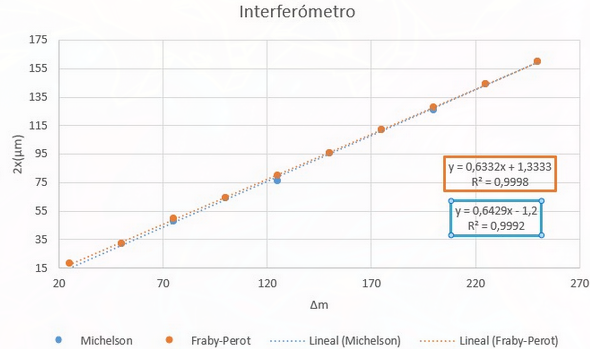
\includegraphics[width=0.8\textwidth]{img/graficaint.png}
    \caption{Vemos en la gráfica los dos interferómetros representados para calcular $\lambda$ mediante el método de mínimos cuadrados.}
    \label{fig:}
\end{figure}

\begin{figure}[H]
    \centering
    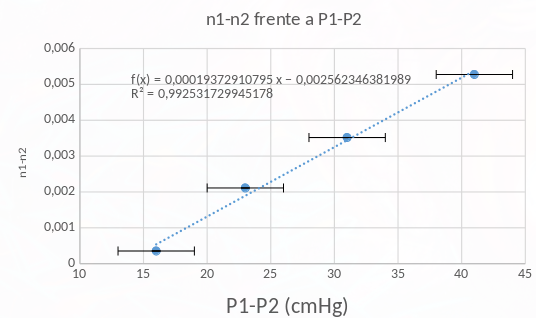
\includegraphics[width=0.8\textwidth]{img/graficap21.png}
    \caption{Representación eliminando el punto que no entraba en la recta de regresión}
    \label{fig:}
\end{figure}    

\begin{figure}[H]
    \centering
    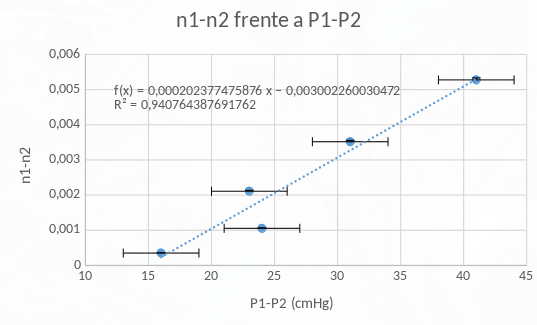
\includegraphics[width=0.8\textwidth]{img/graficap2.png}
    \caption{Representación gráfica para hallar el valor de $m$ }
    \label{fig:img-graficap2-png}
\end{figure}

\onecolumn
\section{Anexo}%
\begin{itemize}
    \item Cálculo de la media ponderada 
\begin{table}[H]
    \centering
    \begin{tabular}{|c|c|c|c|c|c|}
        \hline
        $\lambda=\frac{2x}{\Delta m}$ & $\frac{1}{\Delta \lambda ^2}$ & $\frac{\lambda}{\left( \Delta \lambda \right) ^2}$ & $\lambda =\frac{2x}{\Delta m}$ & $\frac{1}{\Delta \lambda ^2}$ & $ \frac{\lambda}{\left( \Delta \lambda  \right) ^2}$ \\ \hline
        0.56 & 12.7551 & 7.142 & 0.72 & 7.71604 & 5.555 \\ 
        0,64 & 9,765625 & 6,25 & 0,64 & 9,765625 & 6,25 \\
        0,64 & 9,765625 & 6,25 & 0,67 & 9 & 6 \\ 
        0,64 & 9,765625 & 6,25 & 0,64 & 9,765625 & 6,25 \\
        0,608 & 10,820 & 6,5785 & 0,64 & 9,765625 & 6,25 \\
        0,64 & 9,765625 & 6,25 & 0,64 & 9,765625 & 6,25 \\ 
        0,64 & 9,765625 & 6,25 & 0,64 & 9,765625 & 6,25 \\
        0,63 & 10,078106 & 6,3435 & 0,64 & 9,765625 & 6,25 \\
        0,64 & 9,765625 & 6,25 & 0,64 & 9,765625 & 6,25 \\
        0,64 & 9,765625 & 6,25 & 0,64 & 9,765625 & 6,25 \\ \hline
        $\Sigma$ & 102,013 & 63,8245 & $\Sigma$ & 94,8461 & 61,556 \\ \hline
        M.Ponde & 0,6256 &  & M.Ponde & 0,649 &  \\ \hline 
        Error & 0,0990 &  & Error & 0,102 &  \\ \hline
    \end{tabular}
    \label{}
\end{table}

\item Cálculo del error de $  n_1-n_2$ mediante dispersión de Gauss:
\[
    \Delta \left( n_1-n_2 \right) =\sqrt{\left( \frac{N}{2d} \right) ^2\left( \Delta  \lambda \right) ^2 + \left( \frac{N\lambda}{4d^2} \right) ^2\left( \Delta d \right) ^2} 
.\] 
\item Tabla de valores de medida del índice de refracción del aire en función de la presión:
\begin{table}[H]
    \caption{Tabla de valores parte 2 }
    \centering
    \begin{tabular}{|c|c|c|c|c|c|}
        \hline
        N & $ P_1 \pm 2  $ cmHg & $ P_2 \pm 2 $cmHg & $ P_1-P_2 \pm 3  $ cmHg  & $n_1-n_2$ & $\Delta \left( n_1-n_2 \right) $ \\ \hline
        25 & 0 & 16 & 16  & $3.52\cdot 10^{-4}$ & $9 \cdot 10^{-6}$ \\ 
        50 & 16 & 24 & 24  & $1.0053\cdot 10^{-3}$ & $1.6 \cdot 10^{-6}$\\
        75 & 24 & 23 & 23 & $2.11 \cdot 10^{-3}$ & $3 \cdot 10^{-4}$\\
        100 & 32 & 40 & 31  & $3.52\cdot 10^{-3}$ & $4 \cdot 10^{-4}$\\
        125 & 40 & 50 & 41  & $5.28\cdot 10^{-3}$ & $6 \cdot 10^{-4}$\\ \hline
    \end{tabular}
    \label{}
\end{table}

\end{itemize}
\end{document}
